\section{Introduction}
\label{sec:introduction}

Modern vision architectures have diverged rapidly in structural design: vision transformers use layer normalization and global self-attention~\cite{touvron2021training}, hybrid architectures combine depthwise separable convolutions with layer normalization~\cite{liu2022convnet}, while classical CNNs retain batch normalization~\cite{he2016deep}. Yet optimizer selection has not adapted accordingly; practitioners still default to AdamW or SGD regardless of these structural differences, treating optimizer choice as secondary to architecture and data.

This neglect is consequential. SGD collapses to $11.51\%$ accuracy on layer-normalized ConvNeXt-T while achieving $69.50\%$ on batch-normalized ResNet-50, suggesting normalization type as a critical factor, a hypothesis we later confirm causally (Section~\ref{sec:spectral_analysis}). The same task remains accessible to other optimizers, revealing that the optimizer-architecture interaction is not a minor hyperparameter issue but a fundamental compatibility constraint that current practice ignores.

Why do some optimizers transfer across architectures while others catastrophically fail? Existing first-order methods (AdamW with diagonal curvature estimates, SGD with raw gradient direction) do not explicitly account for how architectural design reshapes the spectral properties of weight gradients. Prior optimizer comparisons typically evaluate single architectures~\cite{schmidt2021crowdedvalley} or lack controlled protocol isolation~\cite{choi2020optimizers}, making it impossible to disentangle optimizer capability from recipe engineering.

We hypothesize that optimizers exploiting \emph{weight-matrix spectral structure}, through Newton--Schulz orthogonalization or Kronecker-factored preconditioning~\cite{bernstein2024old}, should exhibit architecture-robust performance precisely because they adapt to the spectral geometry regardless of how normalization and layer composition reshape the spectral geometry. We test this through a controlled study of three spectral optimizers (Muon~\cite{jordan2024muon}\footnote{At the time of writing, the Muon reference is a blog post and has not been peer-reviewed.}, SOAP~\cite{vyas2025soap}, Shampoo~\cite{gupta2018shampoo}) against AdamW~\cite{loshchilov2019decoupled} and SGD, spanning three architecture families, three datasets, and two training horizons, with independently tuned learning rates per optimizer-architecture pair (Section~\ref{sec:optim_protocol}).

Our experiments reveal three main findings. First, spectral optimization is a \emph{family-level} property: all three methods outperform AdamW by $+9$ to $+16$ percentage points on CIFAR-100 where all were evaluated, with Muon maintaining its advantage ($+5.9$ to $+24.3$\,pp) across all three datasets. Second, the advantage is architecture-dependent (largest on layer-normalized networks, smallest on batch-normalized ones), suggesting normalization type mediates how spectral preconditioning benefits optimization. Third, spectral methods reach near-ceiling accuracy within 20 epochs, surpassing AdamW's 50-epoch performance at roughly half the wall-clock cost.

\paragraph{Contributions.}
\begin{itemize}[leftmargin=*,nosep]
\item The first controlled empirical validation of the spectral optimizer family hypothesis~\cite{bernstein2024old}: all three methods (Muon, SOAP, Shampoo) confer a consistent advantage across three vision architectures and three datasets, establishing optimizer-architecture coupling as a structural design concern.
\item Causal evidence that the spectral advantage is mediated by normalization type: replacing BatchNorm with LayerNorm on ResNet-50 collapses AdamW by ${\sim}17$\,pp while Muon is unaffected, and layer-wise stable-rank-divergence correlations reverse sign between CNNs ($\rho{=}{+}0.45$) and transformers ($\rho{=}{-}0.40$).
\item Practical guidance: spectral methods are architecture-robust candidates across the training conditions tested, achieving superior accuracy at substantially lower training cost.
\end{itemize}

\begin{figure*}[t]
\centering
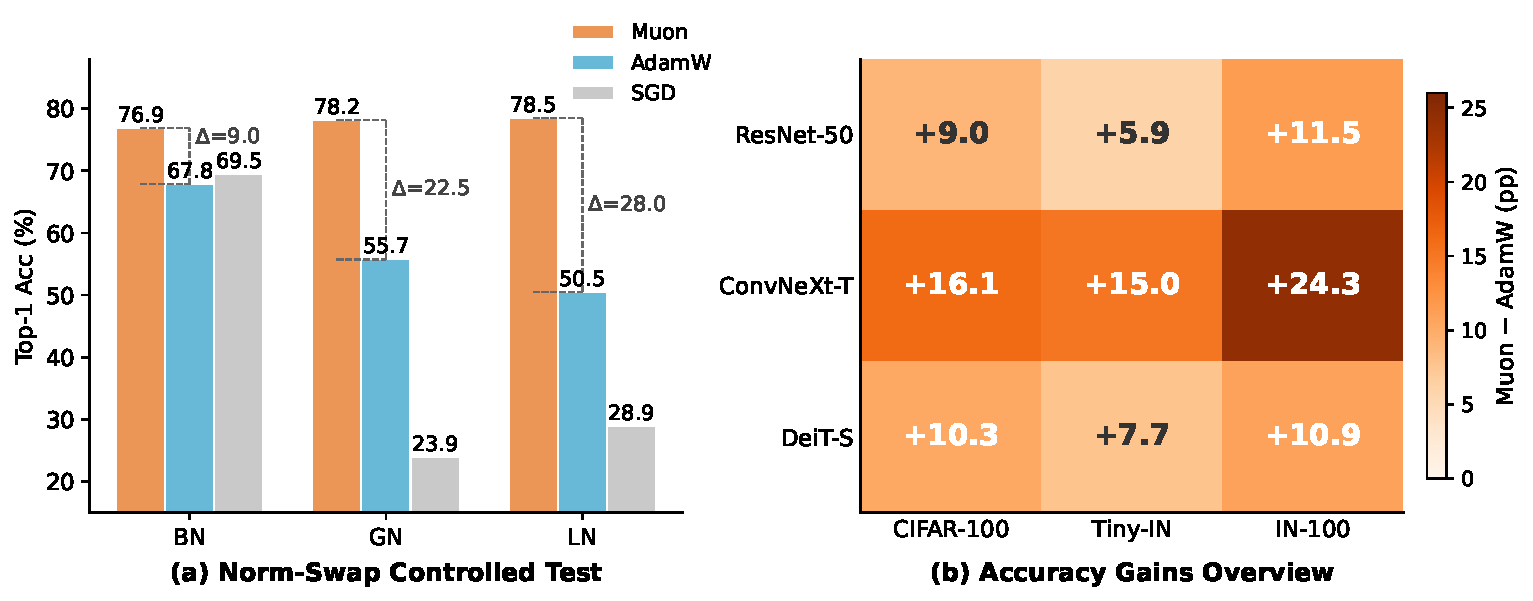
\includegraphics[width=0.88\textwidth]{figures/hero_figure_v6.pdf}
\caption{Overview of spectral optimization advantages in vision tasks. (a) Controlled norm-swap experiment: Muon's advantage persists across BatchNorm, GroupNorm, and LayerNorm ($\Delta < 2$\,pp), while AdamW degrades sharply without BatchNorm. (b) Accuracy gains (Muon $-$ AdamW, pp) across architectures and datasets.}
\label{fig:overview}
\end{figure*}
